
\documentclass[table]{beamer}

\mode<presentation> {
\usetheme{Madrid}

% changes the colors of your current slide theme.

%\usecolortheme{albatross}
%\usecolortheme{beaver}
%\usecolortheme{beetle}
%\usecolortheme{crane}
%\usecolortheme{dolphin}
%\usecolortheme{dove}
%\usecolortheme{fly}
%\usecolortheme{lily}
%\usecolortheme{orchid}
%\usecolortheme{rose}
%\usecolortheme{seagull}
%\usecolortheme{seahorse}
%\usecolortheme{whale}
%\usecolortheme{wolverine}

%\setbeamertemplate{footline} % To remove the footer line in all slides uncomment this line
%\setbeamertemplate{footline}[page number] % To replace the footer line in all slides with a simple slide count uncomment this line

%\setbeamertemplate{navigation symbols}{} % To remove the navigation symbols from the bottom of all slides uncomment this line
}

\usepackage{graphicx} % Allows including images
\usepackage{booktabs} % Allows the use of \toprule, \midrule and \bottomrule in tables
\usepackage{pifont}
\usepackage[english]{babel}
\usepackage{amssymb}
\usepackage{amsmath}
\usepackage[most]{tcolorbox}
%----------------------------------------------------------------------------------------
%	TITLE PAGE
%----------------------------------------------------------------------------------------

\title[Thesis Defense]{Managing Pending Events In Sequential and Optimistic Parallel Discrete Event Simulations} % The short title appears at the bottom of every slide, the full title is only on the title page

\author{Julius D. Higiro} 
\institute[MU]
{
Miami University 
\medskip
}
\date{\today} 

\begin{document}

\begin{frame}
\titlepage 
\end{frame}

\begin{frame}
\frametitle{Overview} 
\tableofcontents 
\end{frame}
\section{Introduction/Motivation}
\section{Background}
\section{Methodology}
\section{GSA results}
\section{Sequential simulation results}
\section{Parallel simulation assessments}
\section{Conclusion and Future Work}


\begin{frame}
\frametitle{\centerline{Introduction}}
\begin{itemize}
\item \textbf{Discrete Event Simulation (DES)} is used to simulate systems of interacting objects.
\item The objects in the simulation are referred to as logical processes (LPs) and model objects in the real world.
\item LPs interact by exchanging time stamped events and process events in priority order with event priorities determined by their time stamp.
\item Events that have yet to be processed are called "\textbf{pending events}".
\item Data structures for handling pending events follow a priority queue based implementation.
\end{itemize}
\end{frame}


\begin{frame}
\frametitle{\centerline{Research Motivation}}
\begin{itemize}
\item Data structures for managing and prioritizing pending events play a critical role in ensuring efficient sequential and parallel simulations.
\item The synchronization strategy in PDES can also impact the effectiveness of data structure because of the additional processing required during rollback recovery operations.
\item A data structure that can effectively handle large number of concurrent events (\textbf{i.e. an average of one million events}).
\end{itemize}
\end{frame}


\begin{frame}
\frametitle{\centerline{Related Work}}
\begin{itemize}
\item Dickman et al., compared event list data structures that consisted of Splay Tree, STL Multiset and Ladder Queue. However, the focus of their paper was in developing a framework for handling pending event set data structure in shared memory PDES. A central component of their study was the identification of an appropriate data structure and design for the shared pending event set.

\item Gupta et al., extended their implementation of Ladder Queue for shared memory Time Warp based simulation environment, so that it supports lock-free access to events in the shared pending event set. The modification involved the use of an unsorted lock-free queue in the underlying Ladder Queue structure.

\item Marotta et al., have contributed to the study of pending event set data structures in threaded PDES through the design of the Non-Blocking Priority Queue (NBPQ) data structure. A pending event set data structure that is closely related to Calendar Queues with constant time performance.
\end{itemize}
\end{frame}


\begin{frame}
\frametitle{\centerline{Thesis}}
\begin{itemize}
\item \textbf{Thesis statement}: Multi-tier data structures (\textbf{2tLadderQ} and \textbf{3tHeap}) outperform all other data structures in sequential and optimistic parallel simulations.
\end{itemize}
\begin{itemize}
\item \textbf{Contribution:}
\setlength{\itemindent}{0.1em}
\item[\ding{182}]\textbf{3-Tier Heap.} \item[\ding{183}]\textbf{2-Tier Ladder Queue (extension of Ladder Queue).} 
\item[\ding{184}]\textbf{Identification of influential model characteristics for choice of \hspace{1mm}queue.} 
\end{itemize}
\end{frame}


\begin{frame}
\frametitle{\centerline{Overview}}
\begin{itemize}
\item[\ding{182}] Introduction/Motivation
\item[\ding{183}] \colorbox{red}{Background}
\item[\ding{184}] Methodology
\item[\ding{185}] GSA results
\item[\ding{186}] Sequential simulation results
\item[\ding{187}] Parallel simulation assessments
\item[\ding{188}]Conclusion and Future Work
\end{itemize}
\end{frame}

\begin{frame}
\frametitle{\centerline{Parallel Simulator Overview}}
\begin{figure}[T]
\begin{minipage}[b]{0.55\textwidth}
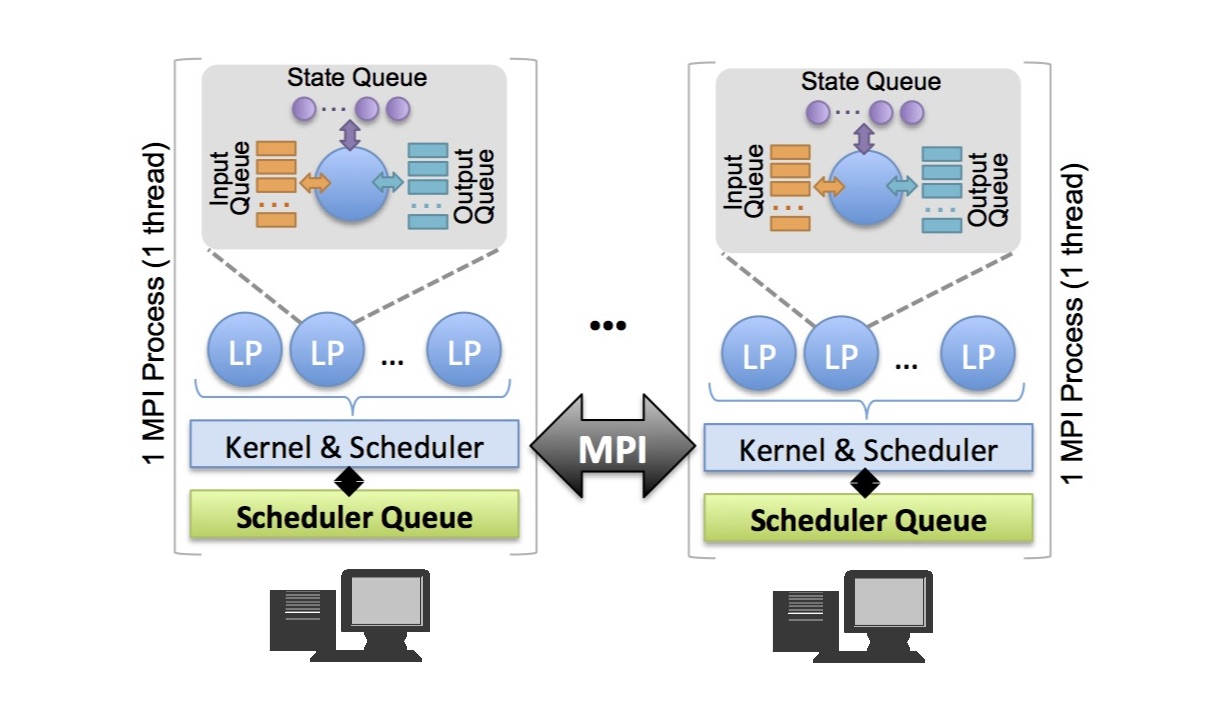
\includegraphics[width=\textwidth]{images/MUSEarch.jpg}
\end{minipage}
\end{figure}
\begin{itemize}
\item Assessment of the data structures was conducted on MUSE.
\item MUSE performs sequential and optimistically parallel simulations.
\item MUSE uses Message Passing Interface (MPI) library for parallel processing.
\item The kernel handles LP registration, event processing, state saving, synchronization and garbage collection.
\end{itemize}
\end{frame}


\begin{frame}
\frametitle{\centerline{Parallel Simulator Overview}}
A scheduler queue is required to implement four key operations to manage pending events. \\~\\
\begin{itemize}
\item[\ding{182}] \textbf{Enqueue one or more future events}. 
\item[\ding{183}] \textbf{Peek next event in priority order}.
\item[\ding{184}] \textbf{Dequeue events with the same time stamp for next LP}.
\item[\ding{185}] \textbf{Cancel pending events after a given time}.
\end{itemize}   
\end{frame}


\begin{frame}
\frametitle{ \centerline{Scheduler Queues}}
\begin{itemize}
\item MUSE contains 6 scheduling queues for managing pending events.
\item The queues are classified into two categories: single-tier and multi-tier queues.
\item Single-tier queues use only a single data structure to implement the 4 key operations.
\item Multi-tier queues organizes events into tiers.
\item Each tier is implemented using different data structures.
\end{itemize}
\end{frame}


\begin{frame}
\frametitle{\centerline{Binary Heap (\textbf{heap})}} 
\begin{figure}
\centering
\begin{minipage}{0.45\textwidth}
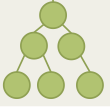
\includegraphics[width=.75\linewidth]{images/binaryHeap.png}
\end{minipage}
\centering
\begin{minipage}{0.45\textwidth}
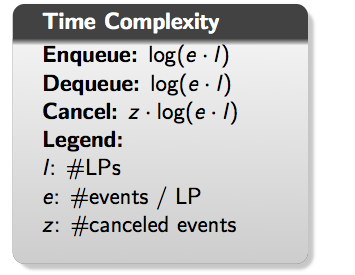
\includegraphics[width=.95\linewidth]{images/complexityHeap.png}
\end{minipage}
\end{figure}
\begin{itemize}
\item It is a single-tier data structure that it is implemented as an array object.
\item A std::vector is used as the backing container and C++11 algorithms (std::push\_heap, st::pop\_heap) are used to maintain the heap.
\item The heap is prioritized based on time stamp with the lowest time stamp at the root of the heap.
\end{itemize}
\end{frame}


\begin{frame}
\frametitle{\centerline{2-tier Heap (\textbf{2tHeap})}}
\begin{figure}
\centering
\begin{minipage}{0.45\textwidth}
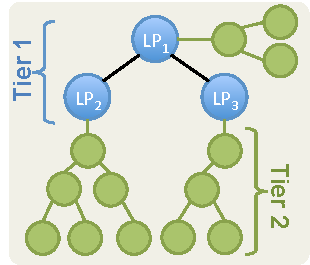
\includegraphics[width=.75\linewidth]{images/2tierQ.pdf}
\end{minipage}
\centering
\begin{minipage}{0.45\textwidth}
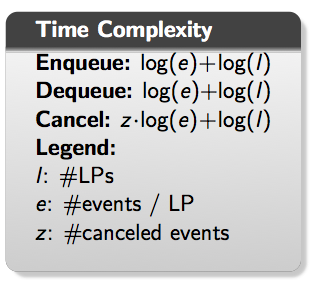
\includegraphics[width=.75\linewidth]{images/complexity2tHeap.png}
\end{minipage}
\end{figure}
\begin{itemize}
\item 2tHeap was designed to reduced the time complexity of cancel operations by subdividing events into two  distinct tiers.
\item The first tier has containers for each local LP on an MPI-process.
\item Each of the the tier-1 containers has a heap of events to be processed by a given LP.
\item A std::vector is used as the backing container for both tiers and standard algorithms are used to maintain the min-heap property for both tiers after each operation.
\end{itemize}
\end{frame}


\begin{frame}
\frametitle{\centerline{2-tier Fibonnaci Heap (\textbf{fibHeap})}}
\begin{figure}
\centering
\begin{minipage}{0.45\textwidth}
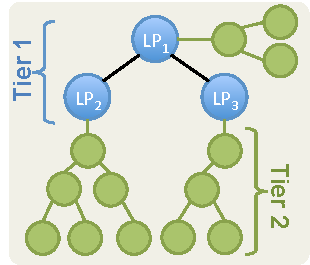
\includegraphics[width=.95\linewidth]{images/2tierQ.pdf}
\end{minipage}
\centering
\begin{minipage}{0.45\textwidth}
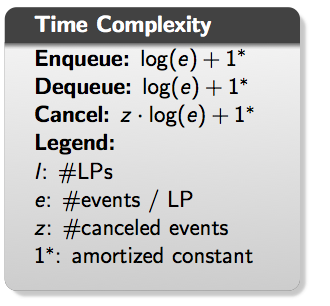
\includegraphics[width=.95\linewidth]{images/complexityfibHeap.png}
\end{minipage}
\end{figure}
\begin{itemize}
\item The fibHeap is an extension of the 2tHeap data structure. It uses a Fibonnaci heap for scheduling LPs.
\item The second tier is a binary heap data structure.
\end{itemize}
\end{frame}


\begin{frame}
\frametitle{\centerline{3-tier Heap (\textbf{3tHeap})}}
\begin{figure}
\centering
\begin{minipage}{0.45\textwidth}
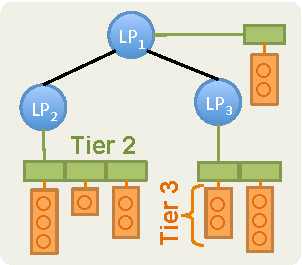
\includegraphics[width=.85\linewidth]{images/3tierQ.pdf}
\end{minipage}
\centering
\begin{minipage}{0.45\textwidth}
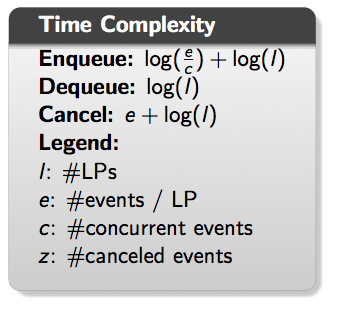
\includegraphics[width=.85\linewidth]{images/complexity3tHeap.png}
\end{minipage}
\end{figure}
\begin{itemize}
\item The 3tHeap builds upon 2tHeap by further subdividing the second tier into two tiers.
\item The binary heap implementation for the first tier that manages LPs for scheduling has been retained from 2tHeap.
\item Assuming each LP has \textit{c} concurrent events on an average, there are $\frac{e}{c}$ tier-2 entries with each one having \textit{c} pending events.
\end{itemize}
\end{frame}


\begin{frame}
\frametitle{\centerline{Ladder Queue (\textbf{ladderQ})}}
\begin{figure}
\centering
\begin{minipage}{0.45\textwidth}
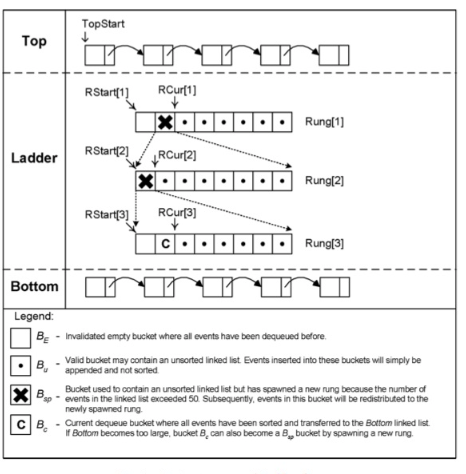
\includegraphics[width=.95\linewidth]{images/LadderQueue.png}
\end{minipage}
\centering
\begin{minipage}{0.45\textwidth}
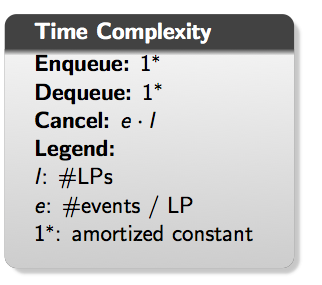
\includegraphics[width=.95\linewidth]{images/complexityLadderQ.png}
\end{minipage}
\end{figure}
\begin{itemize}
\item Ladder Queue is a priority queue implementation proposed by Tang et al. with amortized constant time complexity.
\item There are two key ideas underlying the Ladder Queue, namely: minimize the number of events to be sorted and delay sorting of events as much as possible.
\end{itemize}
\end{frame}


\begin{frame}
\frametitle{\centerline{Ladder Queue (\textbf{ladderQ - Fine Tuned})}}
\begin{figure}
\centering
\begin{minipage}{0.55\textwidth}
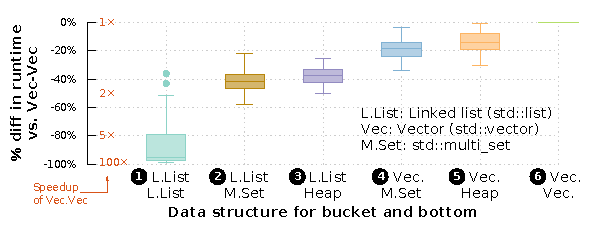
\includegraphics[width=1\linewidth]{images/lq_config_compare.pdf}
\end{minipage}
\centering
\begin{minipage}{0.45\textwidth}
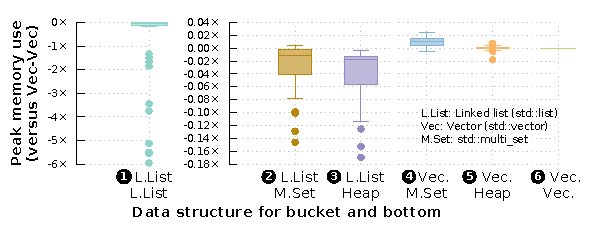
\includegraphics[width=1\linewidth]{images/lq_config_memory_compare.pdf}
\end{minipage}
\end{figure}
\begin{itemize}{\vspace*{-5mm}}
\item Comparison of execution time and peak memory using 6 different ladderQ configurations.
\item L.List-L.List configuration was slowest and performed 85x slower than the Vec-Vec configuration.
\item The increased performance of Vec-Vec comes at about a 6x increase in peak memory footprint when compared to L.List-L.List.
\end{itemize}
\end{frame}


\begin{frame}
\frametitle{\centerline{2-tier Ladder Queue (\textbf{2tLadderQ})}}
\begin{figure}
\centering
\begin{minipage}{0.45\textwidth}
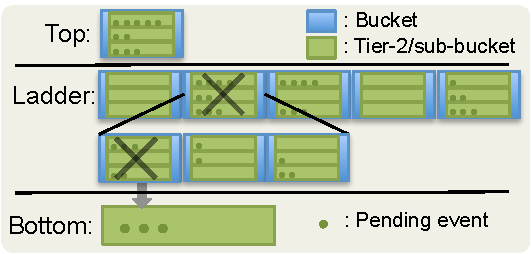
\includegraphics[width=0.99\linewidth]{images/2tLadderQ.pdf}
\end{minipage}
\centering
\begin{minipage}{0.45\textwidth}
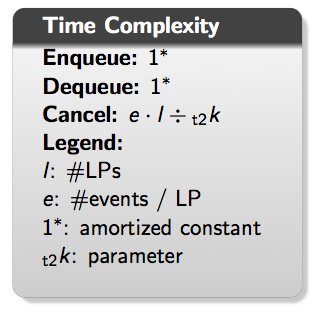
\includegraphics[width=.85\linewidth]{images/complexity2tLadderQ.png}
\end{minipage}
\end{figure}
\begin{itemize}
\item 2-tier Ladder Queue is the proposed alternative to Ladder Queue because the cost of event cancellation during rollbacks is reduced.
\item 2tLadderQ retains the amortized constant time complexity of ladderQ with performance gains during event cancellation.
\end{itemize}
\end{frame}


\frametitle{\centerline{Time Complexity Comparison}}
\begin{frame}	
\begin{table}[!h]
  \caption{Comparison of algorithmic time complexities of different
    data structures}

  Legend -- $l$: \#LPs, $e$: \#events / LP, $c$: \#concurrent events,
  
  $z$: \# canceled events, \textsubscript{t2}\textit{k}: parameter, $1^{*}$: amortized constant
  
  \begin{tabular}{lccc}
    \toprule
    Name & Enqueue & Dequeue & Cancel \\
    \midrule
    \textbf{heap}    & $\log(e\cdot l)$ & $\log(e\cdot l)$ & $z\cdot\log(e\cdot l)$ \\

    \textbf{2tHeap}  & $\log(e) + $ & $\log(e) + $ & $z\cdot\log(e) + $ \\
                & $\log(l)$ & $ \log(l)$      & $ \log(l)$ \\

    \textbf{fibHeap} & $\log(e) + 1^{*}$ & $\log(e) + 1^{*}$ & $z\cdot\log(e) + 1^{*}$ \\

    \textbf{3tHeap}  & $\log(\frac{e}{c}) + \log(l)$ & $\log(l)$ & $e + \log(l)$ \\
    
    \textbf{ladderQ} & $1^{*}$ & $1^{*}$ & $e\cdot l$ \\

    \textbf{2tLadderQ} & $1^{*}$ & $1^{*}$ & $e\cdot l \div$ \textsubscript{t2}\textit{k} \\
    
    \bottomrule
  \end{tabular}
\end{table}
\end{frame}


\begin{frame}
\frametitle{\centerline{Simulation Model - PHOLD}}
\begin{table}[!ht]\centering \vspace*{-4mm}
\textbf{\caption{Parameters in PHOLD benchmark}}
\begin{tabular}{lp{2.2in}}
\toprule
Parameter & Description \\
\midrule
\textbf{rows} & Total number of rows in model. \\
\textbf{cols} & Total number of columns in model. \#LPs = \textbf{rows} x  \textbf{cols} \\
\textbf{eventsPerLP} & Initial number of events per LP. \\
\textbf{delay} or $\lambda$ & Value used with distribution -- Lambda
($\lambda$) value for exponential distribution \textit{i.e.,}
$P(x|\lambda)=\lambda e^{-\lambda x}$. \\
\textbf{\%selfEvents} & Fraction of events LPs send to self \\
\textbf{granularity} & Additional compute load per event. \\
\textbf{imbalance} & Fractional imbalance in partition to have more LPs on a MPI-process. \\
\textbf{simEndTime} & GVT when simulation logically ends.\\
\bottomrule
\end{tabular}
\end{table}
\end{frame}


\begin{frame}
\frametitle{\centerline{PHOLD - Key Parameters}}
\begin{figure}[T]
\begin{minipage}[b]{1\textwidth}
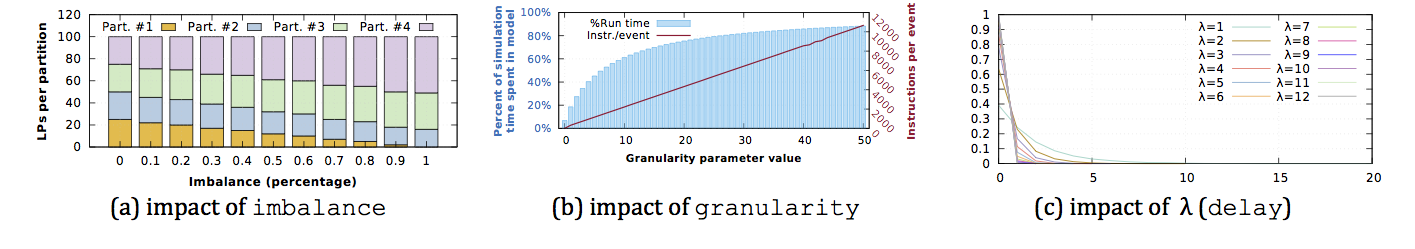
\includegraphics[width=\textwidth]{images/keyParameters.png}
\end{minipage}
\end{figure}
\begin{itemize} 
\item Imbalance parameter influences the partition.
\item Granularity impacts the processing time of events.
\item $\lambda$ impacts the distribution of the time stamp values.
\end{itemize}
\end{frame}


\begin{frame}
\frametitle{\centerline{Simulation Model - PCS}}
\begin{table}[!ht]\centering \vspace*{-4mm}
\textbf{\caption{Parameters in PCS simulation model}}
\begin{tabular}{lp{2.2in}}
\toprule
Parameter & Description \\
\midrule
\textbf{rows} & Total number of rows in model. \\
\textbf{cols} & Total number of columns in model. \#Cells/LPs = \textbf{rows} x  \textbf{cols} \\
\textbf{portables} & The portables represents a mobile phone unit that resides at the Cell for a period of time and then moves to one of four neighboring cells. \\
\bottomrule
\end{tabular}
\end{table}
\end{frame}


\begin{frame}
\frametitle{\centerline{Simulation Model - PCS}}
\begin{table}[!ht]\centering \vspace*{-4mm}
\textbf{\caption{Parameters in PCS simulation model}}
\begin{tabular}{lp{2.2in}}
\toprule
Parameter & Description \\
\midrule
\textbf{moveIntervalMean} & Mean value of an exponential random distribution used to generate the time when a portable will move to an adjacent cell.\\
\textbf{callIntervalMean} & Mean value of an exponential random distribution from where the next call timestamp value is determined. \\
\textbf{callDurationMean} &  Mean value  of a poisson distribution used to generate the length/duration of a call to a portable. \\
\bottomrule
\end{tabular}
\end{table}
\end{frame}


\begin{frame}
\frametitle{\centerline{Simulation Model - PCS}}
\begin{table}[!ht]\centering \vspace*{-4mm}
\textbf{\caption{Parameters in PCS simulation model}}
\begin{tabular}{lp{2.2in}}
\toprule
Parameter & Description \\
\midrule
\textbf{\#channels} & The maximum number of channels assigned to each PCS cell. \\
\textbf{imbalance} & Fractional imbalance in partition to have more LPs on a MPI-process. \\
\textbf{simEndTime} & GVT when simulation logically ends.\\
\bottomrule
\end{tabular}
\end{table}
\end{frame}

\begin{frame}
\frametitle{\centerline{Overview}}
\begin{itemize}
\item[\ding{182}] Introduction/Motivation
\item[\ding{183}] Background
\item[\ding{184}] \colorbox{red}{Methodology}
\item[\ding{185}] GSA results
\item[\ding{186}] Sequential simulation results
\item[\ding{187}] Parallel simulation assessments
\item[\ding{188}]Conclusion and Future Work
\end{itemize}
\end{frame}

\begin{frame}
\frametitle{\centerline{Methodology}}
\begin{itemize}
\item Run different configurations of the PHOLD benchmark and PCS simulation in sequential and optimistically parallel simulations.
\\~\\
\item  Identify the most influential parameters that impact performance of the scheduler queues using \textbf{Generalized Sensitivity Analysis}.\\~\\
\item The data to be collected and assessed consists of the following:
\end{itemize}
\begin{itemize}
\setlength{\itemindent}{2em}
\item[\ding{182}]\textbf{simulation run time.} \item[\ding{183}]\textbf{peak memory usage.} 
\item[\ding{184}]\textbf{\# of rollbacks.} 
\item[\ding{185}]\textbf{characteristics of key queue operations.}
\item[\ding{186}]\textbf{\# of network messages exchanged.}
\end{itemize}
\end{frame}

\begin{frame}
\frametitle{\centerline{Overview}}
\begin{itemize}
\item[\ding{182}] Introduction/Motivation
\item[\ding{183}] Background
\item[\ding{184}] Methodology
\item[\ding{185}] \colorbox{red}{GSA results}
\item[\ding{186}] Sequential simulation results
\item[\ding{187}] Parallel simulation assessments
\item[\ding{188}]Conclusion and Future Work
\end{itemize}
\end{frame}

\begin{frame}
\frametitle{\centerline{Summary of GSA sequential results}}
\begin{itemize}
\item \textbf{Events per LP} - parameter with most influence using \textbf{PHOLD} benchmark. 
\item \textbf{lambda} - parameter with marginal influence using \textbf{PHOLD} benchmark. 
\item \textbf{Portables per Cell} - parameter with most influence using \textbf{PCS} simulation. 
\item Model size - marginal influence using \textbf{PCS} simulation. 
\item \textbf{2tLadderQ} performed better or the same when compared to \textbf{ladderQ}, \textbf{2tHeap}, \textbf{fibHeap}, and \textbf{heap}.
\item \textbf{ladderQ} and \textbf{2tLadderQ} performance was almost indistinguishable with \textsubscript{t2}k = 1.
\item \textbf{3tHeap} outperformed \textbf{2tLadderQ} in certain configurations.
\end{itemize}
\end{frame}


\begin{frame}
\frametitle{\centerline{GSA sequential results - PHOLD}}
\begin{figure}[T]
\begin{minipage}[b]{0.55\textwidth}
\centering
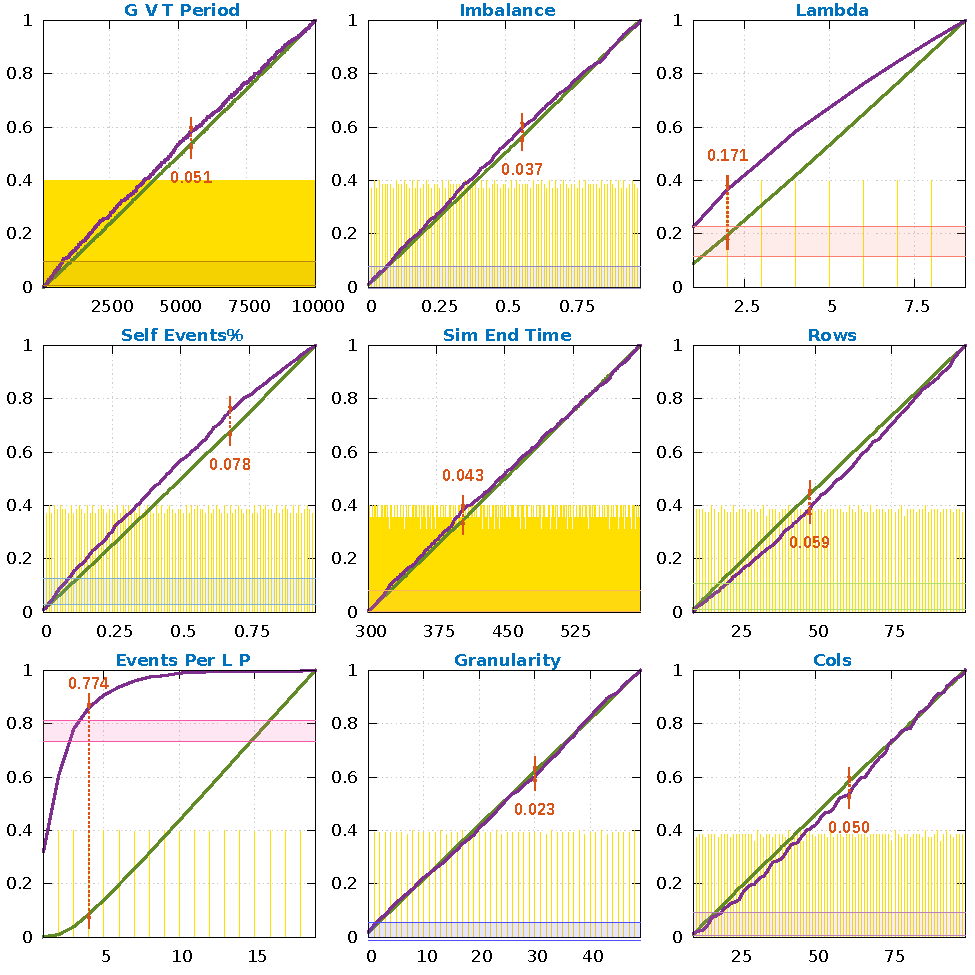
\includegraphics[width=\linewidth]{images/2tlad_vs_3tHeap_gsa.pdf}
\end{minipage}
\textbf{\caption{Results from GSA comparing \textbf{2tLadderQ}
and \textbf{3tHeap} using the PHOLD benchmark.}}
\end{figure}
\end{frame}


\begin{frame}
\frametitle{\centerline{GSA sequential results - PHOLD}}
\begin{figure}[T]
\begin{minipage}[b]{0.95\textwidth}
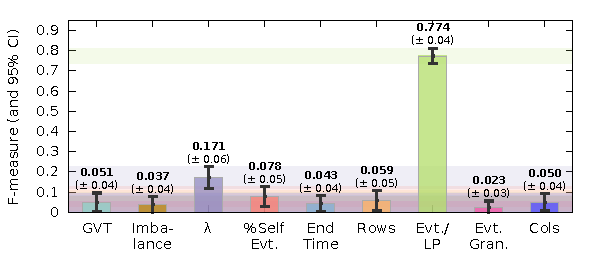
\includegraphics[width=\textwidth]{images/2tlad_vs_3tHeap_gsa_anal_short.pdf}
\end{minipage}
\textbf{\caption{GSA data from sequential simulations (1 MPI-process)
showing influential PHOLD parameters (\textbf{2tLadderQ}
vs. \textbf{3tHeap}).}}
\end{figure}
\end{frame}


\begin{frame}
\frametitle{\centerline{GSA sequential results - PCS}}
\begin{figure}[T]
\begin{minipage}[b]{0.57\textwidth}
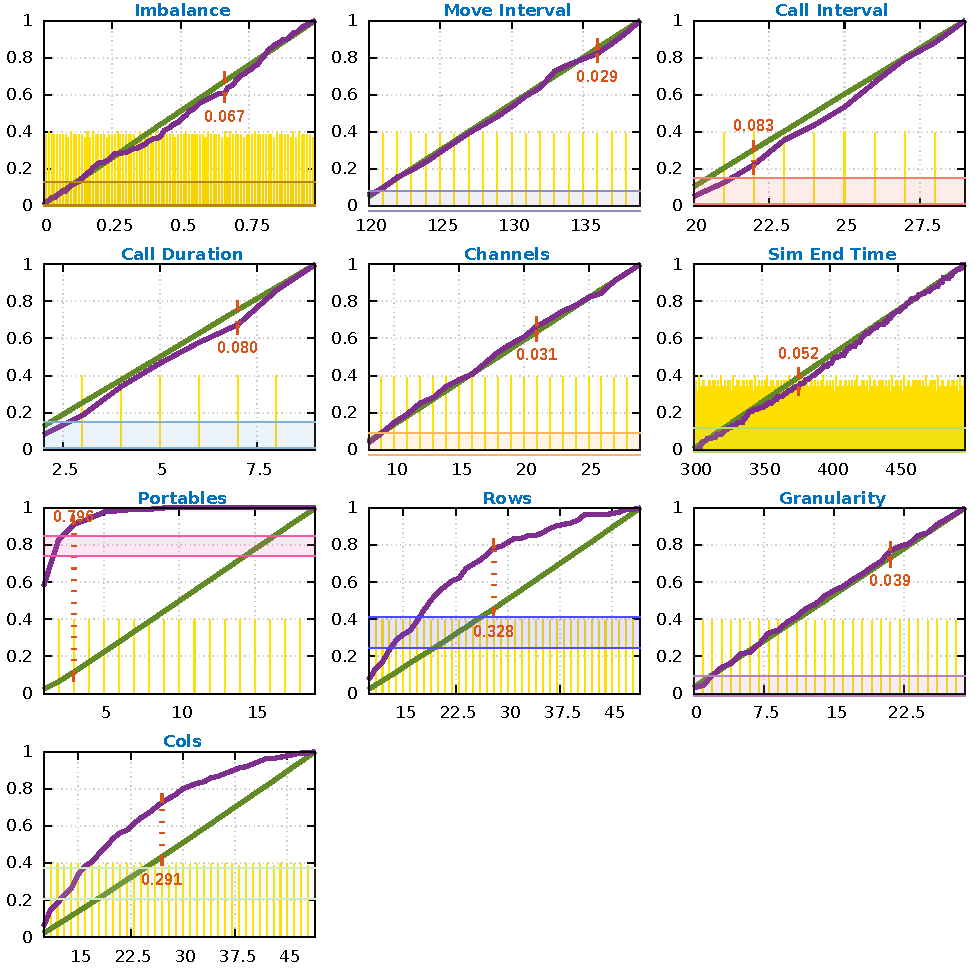
\includegraphics[width=\linewidth]{images/full_gsa_2tladv3tHeapPCS.pdf}
\end{minipage}
\textbf{\caption{Results from GSA comparing \textbf{2tLadderQ}
and \textbf{3tHeap} for sequential simulation using PCS simulation.}}
\end{figure}
\end{frame}


\begin{frame}
\frametitle{\centerline{GSA sequential results - PCS}}
\begin{figure}[T]
\begin{minipage}[b]{0.95\textwidth}
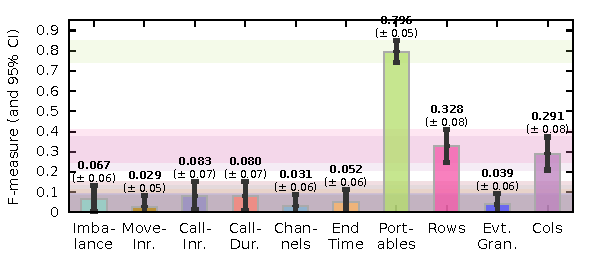
\includegraphics[width=\textwidth]{images/2tLadderQv3tHeapgsa_anal_shortPCS.pdf}
\end{minipage}
\textbf{\caption{GSA data from sequential simulations (1 MPI-process)
showing influential PCS parameters (\textbf{2tLadderQ}
vs. \textbf{3tHeap}).}}
\end{figure}
\end{frame}


\begin{frame}
\frametitle{\centerline{Summary of GSA parallel results}}
-GSA parallel simulations focused on \textbf{ladderQ}, \textbf{2tLadderQ} and \textbf{3tHeap}.
-Parallel results are nearly consistent with sequential results.\\~\\
\begin{itemize}
\item \textbf{Events per LP} - parameter with most influence using \textbf{PHOLD} benchmark. 
\item \textbf{\%Self-Events} - parameter has more pronounced influence in comparison with \textbf{lambda} using \textbf{PHOLD} benchmark. 
\item \textbf{Portables per Cell} - parameter with most influence using \textbf{PCS} simulation. 
\item Model size - marginal influence using \textbf{PCS} simulation. 
\end{itemize}
\end{frame}


\begin{frame}
\frametitle{\centerline{GSA parallel results - PHOLD}}
\begin{figure}[T]
\begin{minipage}[b]{0.95\textwidth}
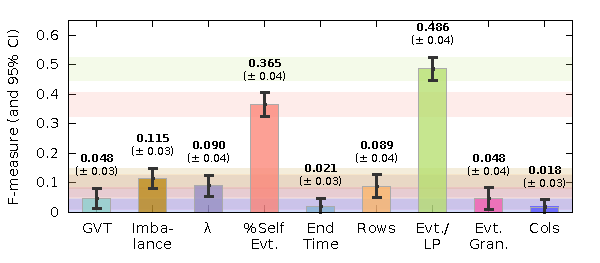
\includegraphics[width=\textwidth]{images/par_2tlad_vs_3tHeap_gsa_anal_short.pdf}
\end{minipage}
\textbf{\caption{GSA data from parallel simulations (4 MPI-processes)
showing influential PHOLD parameters (\textbf{2tLadderQ}
vs. \textbf{3tHeap}).}}
\end{figure}
\end{frame}


\begin{frame}
\frametitle{\centerline{GSA parallel results - PCS}}
\begin{figure}[T]
\begin{minipage}[b]{0.95\textwidth}
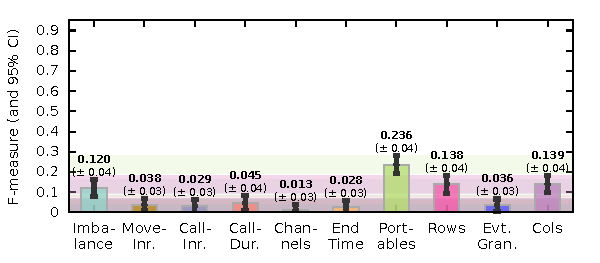
\includegraphics[width=\textwidth]{images/par2tLadderQv3tHeapgsa_anal_shortPCS.pdf}
\end{minipage}
\textbf{\caption{GSA data from parallel simulations (4 MPI-processes)
showing influential PCS parameters (\textbf{2tLadderQ}
vs. \textbf{3tHeap}).}}
\end{figure}
\end{frame}


\begin{frame}
\frametitle{\centerline{Configuration for further analysis}}
\begin{table}[htbp]\centering
\textbf{\caption{Configurations of PHOLD and PCS}\label{tab:configs}}
\begin{tabular}{llll}
\toprule
Name & \#LPs & \multicolumn{2}{c}{Sim. End Time} \\ \cline{3-4}
& (Rows x Cols) & Seq & Parallel \\
\midrule

\textbf{ph3} & 1,000 (100 x 10) & 5000 & 20000 \\

\textbf{ph4} & 10,000  (100 x 100) & 500 & 5000 \\

\textbf{ph5} & 100,000 (1000 x 100) & 100 & 1000 \\

\midrule

\textbf{pcs6} & 100 (10 x 10) & 5000 & 50000 \\

\textbf{pcs7} & 1,000  (100 x 10) & 1000 & 4500 \\

\textbf{pcs8} & 10,000 (100 x 100) & 100 & 200 \\

\bottomrule
\end{tabular}
\end{table}
\end{frame}


\begin{frame}
\frametitle{\centerline{Overview}}
\begin{itemize}
\item[\ding{182}] Introduction/Motivation
\item[\ding{183}] Background
\item[\ding{184}] Methodology
\item[\ding{185}] GSA results
\item[\ding{186}] \colorbox{red}{Sequential simulation results}
\item[\ding{187}] Parallel simulation assessments
\item[\ding{188}]Conclusion and Future Work
\end{itemize}
\end{frame}

\begin{frame}
\frametitle{\centerline{Sequential simulation results - PHOLD}}
\begin{figure}
\begin{minipage}{0.45\linewidth}
\centering
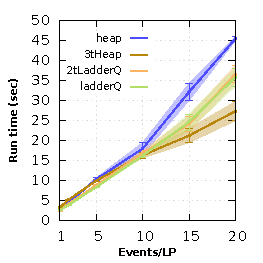
\includegraphics[width=\textwidth]{images/ph3_run_time.pdf}
\end{minipage}
\begin{minipage}{0.45\linewidth}
\centering
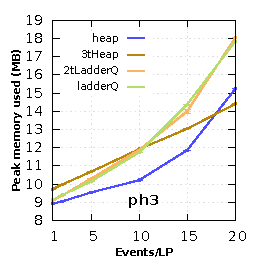
\includegraphics[width=\textwidth]{images/ph3_memory.pdf}
\end{minipage}
\textbf{\caption{Sequential simulation runtimes and peak memory usage with \textbf{ph3}.}}
\end{figure}
\end{frame}


\begin{frame}
\frametitle{\centerline{Sequential simulation results - PHOLD}}

\begin{figure}
\begin{minipage}{0.45\linewidth}
\centering
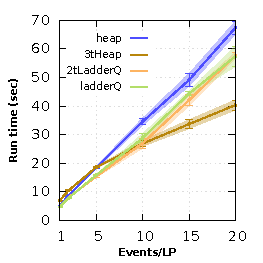
\includegraphics[width=\textwidth]{images/ph4_run_time.pdf}
\end{minipage}
\begin{minipage}{0.45\linewidth}
\centering
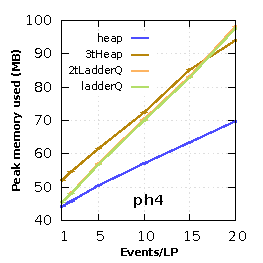
\includegraphics[width=\textwidth]{images/ph4_memory.pdf}
\end{minipage}
\textbf{\caption{Sequential simulation runtimes and peak memory usage with \textbf{ph4}.}}
\end{figure}
\end{frame}



\begin{frame}
\frametitle{\centerline{Sequential simulation results - PHOLD}}
\begin{figure}
\begin{minipage}{0.45\linewidth}
\centering
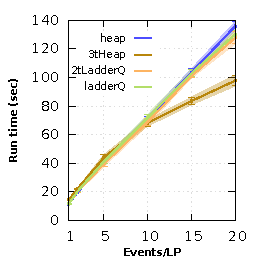
\includegraphics[width=\textwidth]{images/ph5_run_time.pdf}
\end{minipage}
\begin{minipage}{0.45\linewidth}
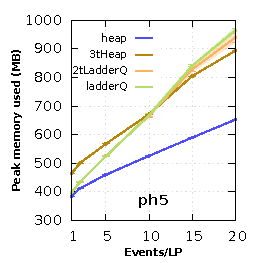
\includegraphics[width=\textwidth]{images/ph5_memory.pdf}
\end{minipage}
\textbf{\caption{Sequential simulation runtimes and peak memory usage with \textbf{ph5}.}}
\end{figure}
\end{frame}



\begin{frame}
\frametitle{\centerline{Sequential simulation results - PCS}}
\begin{figure}
\begin{minipage}{0.49\linewidth}
\centering
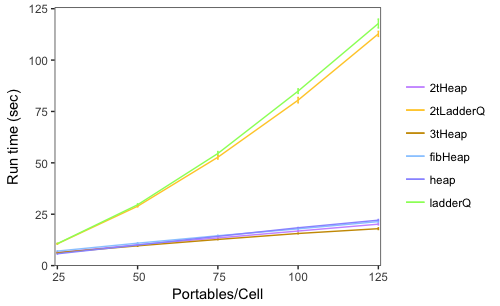
\includegraphics[width=\textwidth]{images/pcs6_runtime_full.png}
\end{minipage}
\begin{minipage}{0.49\linewidth}
\centering
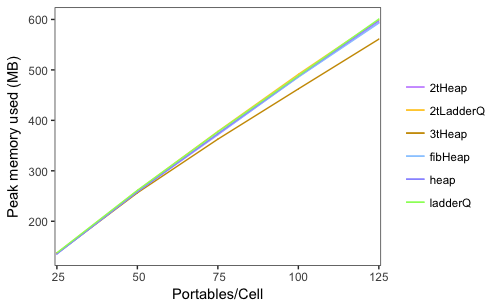
\includegraphics[width=\textwidth]{images/pcs6_memory_full.png}
\end{minipage}
\textbf{\caption{Sequential simulation runtimes and peak memory usage with \textbf{pcs6}.}}
\end{figure}
\end{frame}



\begin{frame}
\frametitle{\centerline{Sequential simulation results - PCS}}
\begin{figure}
\begin{minipage}{0.49\linewidth}
\centering
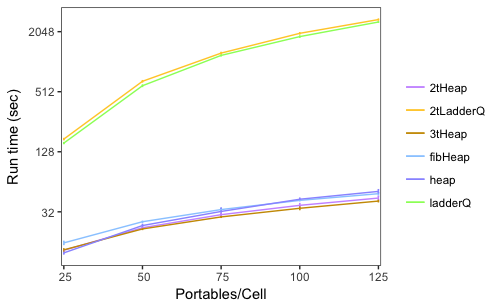
\includegraphics[width=\textwidth]{images/pcs7_runtime_full_log.png}
\end{minipage}
\begin{minipage}{0.49\linewidth}
\centering
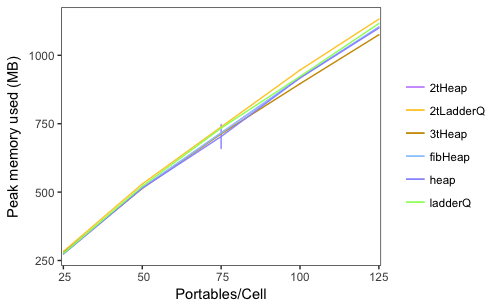
\includegraphics[width=\textwidth]{images/pcs7_memory_full.png}
\end{minipage}
\textbf{\caption{Sequential simulation runtimes and peak memory usage with \textbf{pcs7}.}}
\end{figure}
\end{frame}



\begin{frame}
\frametitle{\centerline{Sequential simulation results - PCS}}
\begin{figure}
\begin{minipage}{0.49\linewidth}
\centering
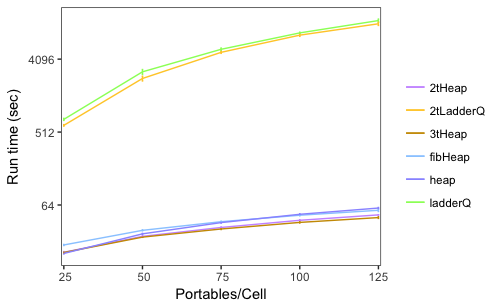
\includegraphics[width=\textwidth]{images/pcs8_runtime_full_log.png}
\end{minipage}
\begin{minipage}{0.49\linewidth}
\centering
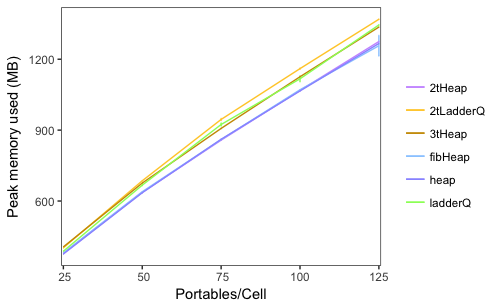
\includegraphics[width=\textwidth]{images/pcs8_memory_full.png}
\end{minipage}
\textbf{\caption{Sequential simulation runtimes and peak memory usage with \textbf{pcs8}.}}
\end{figure}
\end{frame}

\begin{frame}
\frametitle{\centerline{Overview}}
\begin{itemize}
\item[\ding{182}] Introduction/Motivation
\item[\ding{183}] Background
\item[\ding{184}] Methodology
\item[\ding{185}] GSA results
\item[\ding{186}] Sequential simulation results
\item[\ding{187}] \colorbox{red}{Parallel simulation assessments}
\item[\ding{188}]Conclusion and Future Work
\end{itemize}
\end{frame}

\begin{frame}
\frametitle{\centerline{Parallel simulation assessment - Efficient case for \textbf{ladderQ}}}
\begin{figure}
\begin{minipage}{0.45\linewidth}
\centering
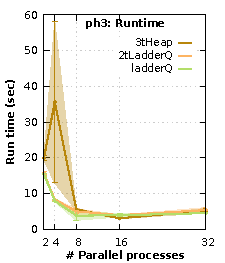
\includegraphics[width=\textwidth]{images/ph3_Delay_1_Evt_2_run_time.pdf}
\end{minipage}
\begin{minipage}{0.45\linewidth}
\centering
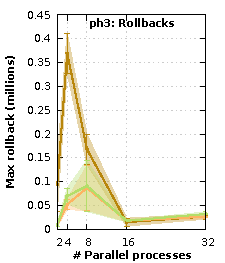
\includegraphics[width=\textwidth]{images/ph3_Delay_1_Evt_2_rollbacks.pdf}
\end{minipage}
\textbf{\caption{Statistics from PH3 configuration of PHOLD parallel simulation with eventsPerLP=2, $\lambda= 1$, \%selfEvents=25\% }}
\end{figure}
\end{frame}

\begin{frame}
\frametitle{\centerline{Parallel simulation assessment - Efficient case for \textbf{ladderQ}}}
\begin{figure}
\begin{minipage}{0.45\linewidth}
\centering
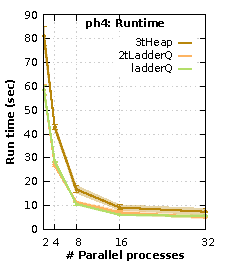
\includegraphics[width=\textwidth]{images/ph4_Delay_1_Evt_2_run_time.pdf}
\end{minipage}
\begin{minipage}{0.45\linewidth}
\centering
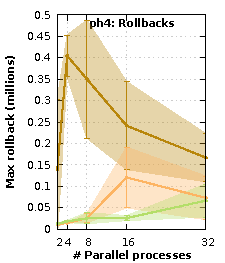
\includegraphics[width=\textwidth]{images/ph4_Delay_1_Evt_2_rollbacks.pdf}
\end{minipage}
\textbf{\caption{Statistics from PH4 configuration of PHOLD parallel simulation with eventsPerLP=2, $\lambda= 1$, \%selfEvents=25\% }}
\end{figure}
\end{frame}


\begin{frame}
\frametitle{\centerline{Parallel simulation assessment - Efficient case for \textbf{ladderQ}}}
\begin{figure}
\begin{minipage}{0.45\linewidth}
\centering
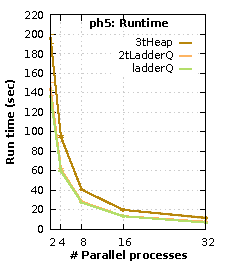
\includegraphics[width=\textwidth]{images/ph5_Delay_1_Evt_2_run_time.pdf}
\end{minipage}
\begin{minipage}{0.45\linewidth}
\centering
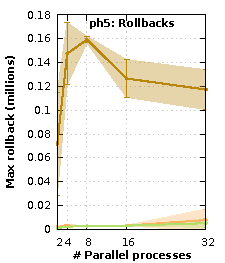
\includegraphics[width=\textwidth]{images/ph5_Delay_1_Evt_2_rollbacks.pdf}
\end{minipage}
\textbf{\caption{Statistics from PH5 configuration of PHOLD parallel simulation with eventsPerLP=2, $\lambda= 1$, \%selfEvents=25\% }}
\end{figure}
\end{frame}



\begin{frame}
\frametitle{Parallel simulation assessment -  Knee point for \textbf{3tHeap} vs. \textbf{ladderQ}}
\begin{figure}
\begin{minipage}{0.45\linewidth}
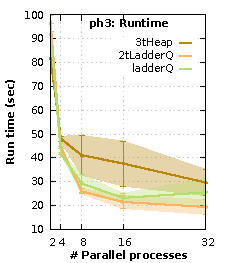
\includegraphics[width=\textwidth]{images/ph3_Delay_10_Evt_10_run_time.pdf}
\end{minipage}
\begin{minipage}{0.45\linewidth}
\centering
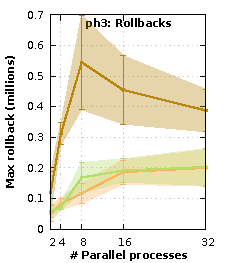
\includegraphics[width=\textwidth]{images/ph3_Delay_10_Evt_10_rollbacks.pdf}
\end{minipage}
\textbf{\caption{Statistics from PH3 configuration of PHOLD parallel simulation with eventsPerLP=10, $\lambda= 10$, \%selfEvents=25\% }}
\end{figure}
\end{frame}


\begin{frame}
\frametitle{Parallel simulation assessment -  Knee point for \textbf{3tHeap} vs. \textbf{ladderQ}}
\begin{figure}
\begin{minipage}{0.45\linewidth}
\centering
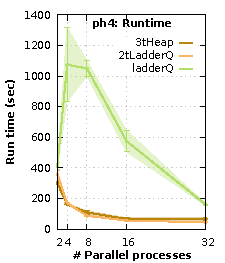
\includegraphics[width=\textwidth]{images/ph4_Delay_10_Evt_10_run_time.pdf}
\end{minipage}
\begin{minipage}{0.45\linewidth}
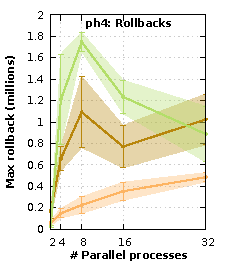
\includegraphics[width=\textwidth]{images/ph4_Delay_10_Evt_10_rollbacks.pdf}
\end{minipage}
\textbf{\caption{Statistics from PH4 configuration of PHOLD parallel simulation with eventsPerLP=10, $\lambda= 10$, \%selfEvents=25\% }}
\end{figure}
\end{frame}


\begin{frame}
\frametitle{Parallel simulation assessment -  Knee point for \textbf{3tHeap} vs. \textbf{ladderQ}}
\begin{figure}
\begin{minipage}{0.45\linewidth}
\centering
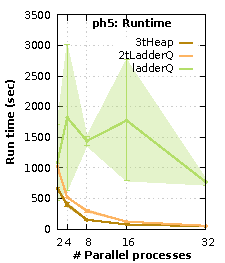
\includegraphics[width=\textwidth]{images/ph5_Delay_10_Evt_10_run_time.pdf}
\end{minipage}
\begin{minipage}{0.45\linewidth}
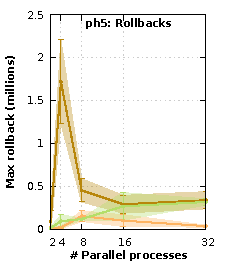
\includegraphics[width=\textwidth]{images/ph5_Delay_10_Evt_10_rollbacks.pdf}
\end{minipage}
\textbf{\caption{Statistics from PH5 configuration of PHOLD parallel simulation with eventsPerLP=10, $\lambda= 10$, \%selfEvents=25\% }}
\end{figure}
\end{frame}


\begin{frame}
\frametitle{\centerline{Parallel simulation assessment - Best case for \textbf{3tHeap}}}
\begin{figure}
\begin{minipage}{0.45\linewidth}
\centering
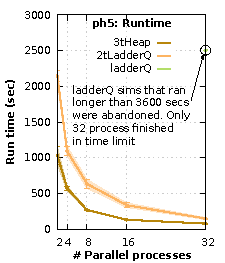
\includegraphics[width=\textwidth]{images/ph5_Delay_10_Evt_20_run_time.pdf}
\end{minipage}
\begin{minipage}{0.45\linewidth}
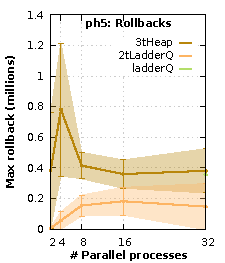
\includegraphics[width=\textwidth]{images/ph5_Delay_10_Evt_20_rollbacks.pdf}
\end{minipage}
\textbf{\caption{Statistics from PH5 configuration of PHOLD parallel simulation with eventsPerLP=20, $\lambda= 10$, \%selfEvents=25\% }}
\end{figure}
\end{frame}


\begin{frame}
\frametitle{\centerline{Parallel simulation assessment - Best case for \textbf{3tHeap}}}
\begin{figure}
\begin{minipage}{0.99\linewidth}
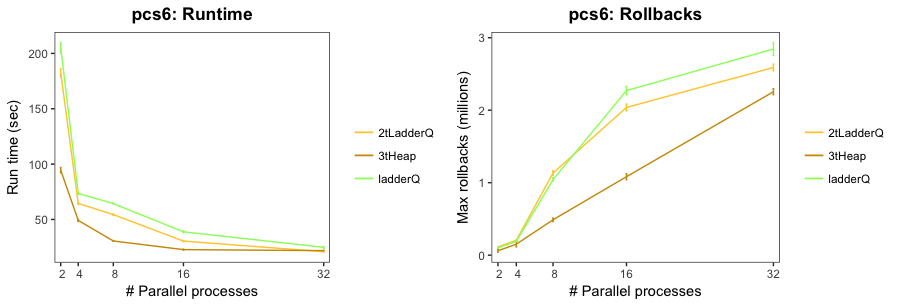
\includegraphics[width=\linewidth]{images/pcs6_parallel_75.png}
\end{minipage}
\textbf{\caption{Statistics from PCS6 configuration of PCS parallel simulation with portables per cell = 75}}
\end{figure}
\end{frame}


\begin{frame}
\frametitle{\centerline{Parallel simulation assessment - Best case for \textbf{3tHeap}}}
\begin{figure}
\begin{minipage}{0.99\linewidth}
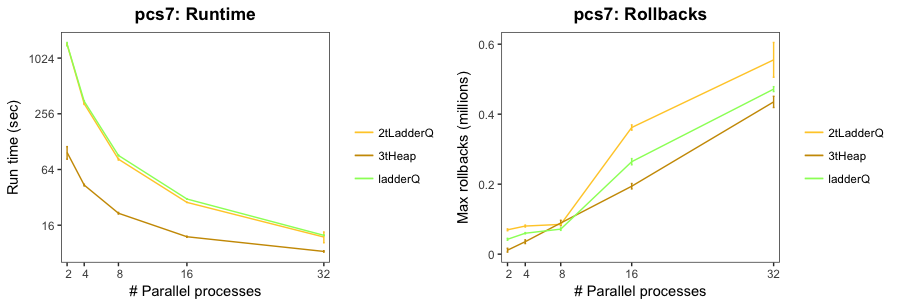
\includegraphics[width=\linewidth]{images/pcs7_parallel_75_log.png}
\end{minipage}
\textbf{\caption{Statistics from PCS7 configuration of PCS parallel simulation with portables per cell = 75}}
\end{figure}
\end{frame}


\begin{frame}
\frametitle{\centerline{Parallel simulation assessment - Best case for \textbf{3tHeap}}}
\begin{figure}
\begin{minipage}{0.99\linewidth}
\includegraphics[width=\linewidth]{images/pcs8_parallel_75_log.png}
\end{minipage}
\textbf{\caption{Statistics from PCS8 configuration of PCS parallel simulation with portables per cell = 75}}
\end{figure}
\end{frame}

\begin{frame}
\frametitle{\centerline{Overview}}
\begin{itemize}
\item[\ding{182}] Introduction/Motivation
\item[\ding{183}] Background
\item[\ding{184}] Methodology
\item[\ding{185}] GSA results
\item[\ding{186}] Sequential simulation results
\item[\ding{187}] Parallel simulation assessments
\item[\ding{188}] \colorbox{red}{Conclusion and Future Work}
\end{itemize}
\end{frame}

\begin{frame}
\frametitle{\centerline{Conclusions}}
\begin{itemize}
\item Recommend the use of General Sensitivity Analysis (GSA) to reduce the parameter space in simulation models with large parameters.
\item \textbf{2tLadderQ} performs no worse than \textbf{ladderQ} in sequential simulations with \textsubscript{t2}k=1. 
\item Results favor the general use of \textbf{2tLadderQ} over the \textbf{ladderQ}.
\item The advantages of \textbf{3tHeap} is realized only when each logical process has 10 or more concurrent events at each time step.
\item Multi-tier data structures perform consistently better in optimistic parallel simulations.
\end{itemize}
\end{frame}

\begin{frame}
\frametitle{\centerline{Future Work}}
\begin{itemize}
\item Implement our multi-tier data structures in a different language and compare performance.
\item Test data structures on other parallel simulation frameworks. 
\item Assess the performance of our data structures using a wider range of simulation models.
\item Assess the effectiveness of multi-tier data structures in multi-threaded simulations.
\end{itemize}
\end{frame}

\begin{frame}
\frametitle{\centerline{References}}
\footnotesize{
\begin{thebibliography}{99}\vspace*{-3.5mm}
\bibitem[Dickman et al., 2013]{p1} Dickman et al., (2013) Event Pool Structures for PDES on Many-core Beowulf Clusters. \emph{In Proceedings of the 1st ACM SIGSIM Conference on Principles of Advanced Discrete Simulation} ACM, New York, NY, USA, 103-114.

\bibitem[Franceschini et al., 2015]{p1} Franceschini et al., (2015) A Comparative Study of Pending Event Set Implementations for PDEVS Simulation. \emph{In Proceedings of the Symposium on Theory of Modeling and Simulation} Society for Computer Simulation International San Diego, CA, USA, 77-84.

\bibitem[Gupta et al., 2014]{p1} Gupta et al., (2014) Lock-free Pending Event Set Management in Time Warp. \emph{In Proceedings of the 2nd ACM SIGSIM Conference on Principles of Advanced Discrete Simulation} ACM, New York, NY, USA, 15-26.

\bibitem[Jafer et al., 2013]{p1} Jafer et al., (2013) Synchronization methods in parallel and distributed discrete-event simulation{ Simulation Modeling Practice and Theory} 30(2013), 54-73.

\bibitem[Marotta et al., 2016]{p1} Marotta et al., (2016) A Non-Blocking Priority Queue for the Pending Event Set.{In Proceedings of the 9th EAI International Conference on Simulation Tools and Techniques} ICST, Brussels, Belgium, 46-55.

\bibitem[Tang et al., 2005]{p1} Tang et al., (2005) Ladder Queue: An O(1) Priority Queue Structure for Large-scale Discrete Event Simulation.{ACM Trans. Model. Comput. Simul.} 15, 3(July 2005), 175-204.
\end{thebibliography}
}
\end{frame}

%------------------------------------------------

\begin{frame}
\Huge{\centerline{The End}}
\end{frame}


\end{document}